\documentclass[10pt]{article}
\usepackage[utf8]{inputenc}
\usepackage[colorlinks]{hyperref}
\usepackage{mathtools, amsthm, thmtools, amsfonts, amssymb,amsmath}
\usepackage{color}
\usepackage{tikz}
\usetikzlibrary{decorations.pathreplacing}

\begin{document}

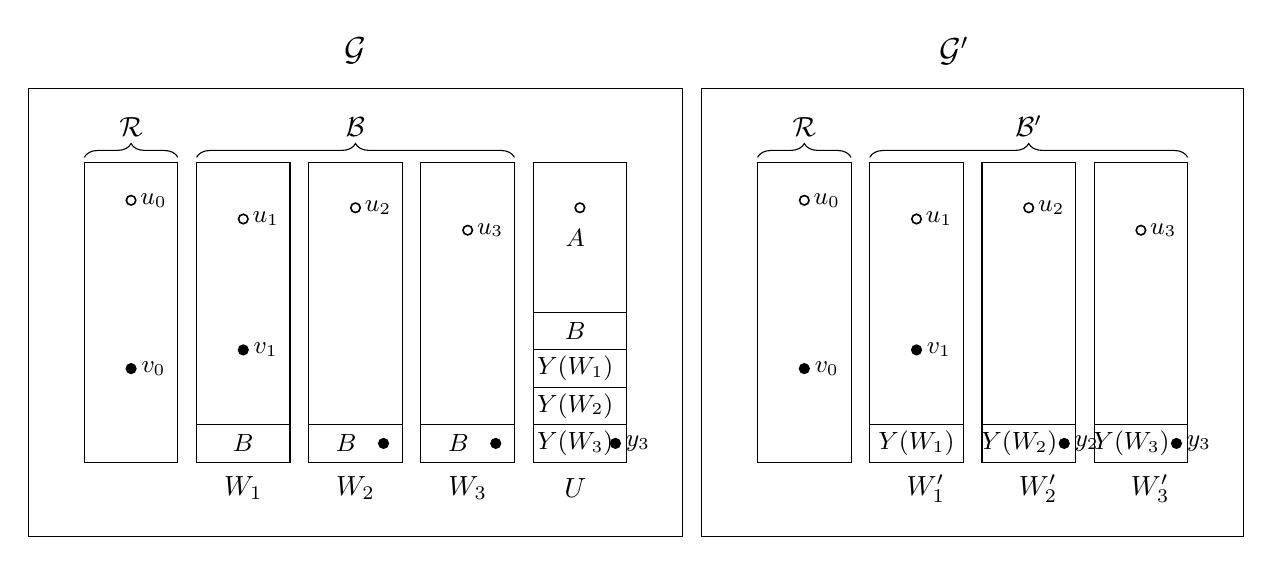
\begin{tikzpicture}[scale=0.95]
    % Rectangles belonging to R
    \draw (0,0) rectangle (1.25,4);
    \draw (-1.5,0) rectangle (-0.25,4);
    \draw (-3,0) rectangle (-1.75,4);
    \draw (-4.5,0) rectangle (-3.25,4);
    \draw (-6,0) rectangle (-4.75,4);
    % Bounding box
    \draw (-6.75,-1) rectangle (2,5);
    \node at (-2.375,5.5) {\large$\mathcal{G}$};

    % Rectangles belonging to R'
    \draw (3,0) rectangle (4.25,4);
    \draw (4.5,0) rectangle (5.75,4);
    \draw (6,0) rectangle (7.25,4);
    \draw (7.5,0) rectangle (8.75,4);
    %Bounding Box
    \draw (2.25,-1) rectangle (9.5,5);
    \node at (5.625,5.5) {\large$\mathcal{G}'$};


    \fill (1.1,0.25) circle (0.075);
    \node at (1.4,0.25) {\small$y_3$};

    %First rectangle
    \draw (0,2) -- (1.25,2);
    \draw (0,0.5) -- (1.25, 0.5);
    \draw (0,1) -- (1.25, 1);
    \draw (0,1.5) -- (1.25, 1.5);
    \node at (0.5625,0.25) {\small$Y(W_3)$};
    \node at (0.5625,0.75) {\small$Y(W_2)$};
    \node at (0.5625,1.25) {\small$Y(W_1)$};
    \node at (0.5625,1.75) {\small$B$};
    \node at (0.5625,3) {\small$A$};
    \node at (0.5625,-0.35) {$U$};

    % Decorations on the B blocks
    \draw (-1.5,0.5) -- (-0.25, 0.5);
    \node at (-1,0.25) {\small$B$};
    \fill (-0.5,0.25) circle (0.075);
    \node at (-0.875,-0.35) {$W_3$};

    \draw (-3,0.5) -- (-1.75, 0.5);
    \node at (-2.5,0.25) {\small$B$};
    \fill (-2,0.25) circle (0.075);
    \node at (-2.375,-0.35) {$W_2$};

    \draw (-4.5,0.5) -- (-3.25, 0.5);
    \node at (-3.875,0.25) {\small$B$};
    \node at (-3.875,-0.35) {$W_1$};
    \fill (-3.875,1.5) circle (0.075);
    \node at (-3.575,1.5) {\small$v_1$};

    \fill (-5.375,1.25) circle (0.075);
    \node at (-5.075,1.25) {\small$v_0$};

    \draw[decorate,decoration={brace,amplitude=5pt,raise=2pt}] (-4.5,4) -- node[above=6pt] {$\mathcal{B}$} (-0.25,4);

    \draw[decorate,decoration={brace,amplitude=5pt,raise=2pt}] (-6,4) -- node[above=6pt] {$\mathcal{R}$} (-4.75,4);

    % Decorations on the B' blocks
    \draw (4.5,0.5) rectangle (5.75,0.5);
    \node at (5.125,0.25) {\small$Y(W_1)$};
    \node at (5.25,-0.35) {$W_1'$};
    \fill (5.125,1.5) circle (0.075);
    \node at (5.425,1.5) {\small$v_1$};


    \fill (3.625,1.25) circle (0.075);
    \node at (3.925,1.25) {\small$v_0$};

    \draw (6,0.5) rectangle (7.25,0.5);
    \node at (6.5,0.25) {\small$Y(W_2)$};
    \fill (7.1,0.25) circle (0.075);
    \node at (7.4,0.25) {\small$y_2$};
    \node at (6.75,-0.35) {$W_2'$};

    \draw (7.5,0.5) rectangle (8.75,0.5);
    \node at (8,0.25) {\small$Y(W_3)$};
    \fill (8.6,0.25) circle (0.075);
    \node at (8.9,0.25) {\small$y_3$};
    \node at (8.25,-0.35) {$W_3'$};

    \draw[decorate,decoration={brace,amplitude=5pt,raise=2pt}] (4.5,4) -- node[above=6pt] {$\mathcal{B}'$} (8.75,4);

    \draw[decorate,decoration={brace,amplitude=5pt,raise=2pt}] (3,4) -- node[above=6pt] {$\mathcal{R}$} (4.25,4);

    % The u transversal in G'
    \fill (3.625,3.5) circle (0.075);
    \fill[white] (3.625,3.5) circle (0.05);
    \node at (3.925,3.5) {\small$u_0$};

    \fill (5.125,3.25) circle (0.075);
    \fill[white] (5.125,3.25) circle (0.05);
    \node at (5.425,3.25) {\small$u_1$};

    \fill (6.625,3.4) circle (0.075);
    \fill[white] (6.625,3.4) circle (0.05);
    \node at (6.925,3.4) {\small$u_2$};

    \fill (8.125,3.1) circle (0.075);
    \fill[white] (8.125,3.1) circle (0.05);
    \node at (8.425,3.1) {\small$u_3$};

    % The u transversal in G
    \fill (-5.375,3.5) circle (0.075);
    \fill[white] (-5.375,3.5) circle (0.05);
    \node at (-5.075,3.5) {\small$u_0$};

    \fill (-3.875,3.25) circle (0.075);
    \fill[white] (-3.875,3.25) circle (0.05);
    \node at (-3.575,3.25) {\small$u_1$};

    \fill (-2.375,3.4) circle (0.075);
    \fill[white] (-2.375,3.4) circle (0.05);
    \node at (-2.075,3.4) {\small$u_2$};

    \fill (-0.875,3.1) circle (0.075);
    \fill[white] (-0.875,3.1) circle (0.05);
    \node at (-0.575,3.1) {\small$u_3$};

    \fill (0.625,3.4) circle (0.075);
    \fill[white] (0.625,3.4) circle (0.05);

\end{tikzpicture}

\end{document}